%META {"question":"Tia Oz nằm trong góc vuông xOy, chia góc vuông thành hai phần bằng nhau. Nếu gọi số đo của mỗi góc nhỏ tạo bởi Oz là k°, khẳng định nào ĐÚNG?","options":["k = 45 — Oz là tia phân giác của góc vuông xOy","k = 90 — Oz là tia phân giác của góc vuông xOy","k = 60 — Oz không là tia phân giác","k = 30 — Oz là tia phân giác"],"answer":0,"note":"Góc vuông bằng 90°; chia đôi thì mỗi góc bằng 45°. Tia nằm giữa hai tia gốc và tạo hai góc bằng nhau (45° = 45°) là tia phân giác."}
\documentclass[border=5pt]{standalone}
\usepackage{tkz-euclide}
% Màu dùng chung cho toàn bộ hình vẽ (ảnh stack với nền tối của web)
\definecolor{tminc}{RGB}{226,232,240}   % chữ + nét chính
\definecolor{tmblue}{RGB}{0,210,255}    % nhấn neon xanh
\definecolor{tmpink}{RGB}{255,0,200}    % nhấn neon hồng
\definecolor{tmgreen}{RGB}{0,255,136}   % nhấn neon xanh lá
\color{tminc}

\begin{document}
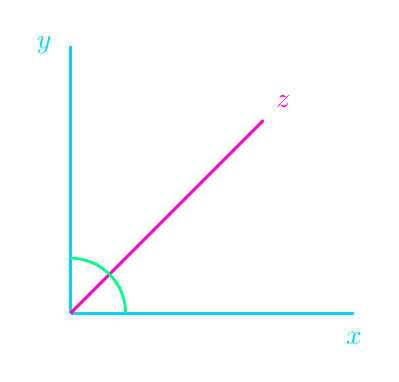
\begin{tikzpicture}[line width=1.1pt]
  \coordinate (O) at (0,0);
  \coordinate (X) at (3.6,0);
  \coordinate (Y) at (0,3.4);
  \coordinate (Z) at (2.45,2.45);
  \draw[tmblue] (O) -- (X) node[below=3pt]{$x$};
  \draw[tmblue] (O) -- (Y) node[left=3pt]{$y$};
  \draw[tmpink] (O) -- (Z) node[above right=1pt]{$z$};
  \tkzMarkAngles[size=0.7,arc=l,color=tmgreen,line width=1pt](X,O,Z)
  \tkzMarkAngles[size=0.7,arc=l,color=tmgreen,line width=1pt](Z,O,Y)
\end{tikzpicture}
\end{document}
